\documentclass{beamer}

\usepackage[brazil]{babel}   
\usepackage[utf8]{inputenc}

\usepackage{lmodern} % Corrige erro de fontsize.

\title{Trabalho da disciplina de Sistemas Evolutivos:\\ A Cellular Automata
 Model of Population Infected by Periodic Plague}

\author{Alexandre Gomes da Costa}

\institute{Centro de Desenvolvimento Tecnológico (CDTec)\\
    Universidade Federal de Pelotas (UFPEL)\\
    Pelotas -- RS -- Brasil\\
    \texttt{alexandre.costa@inf.ufpel.edu.br}
}
  
\begin{document}
% ----------------------------------------------------------------------------
% Slide de Titulo
% ----------------------------------------------------------------------------
\begin{frame} 
\maketitle
\end{frame}

% ----------------------------------------------------------------------------
% Slide de Sumário
% ----------------------------------------------------------------------------
\begin{frame}
\frametitle{Sumário}
\tableofcontents
\end{frame}

% ----------------------------------------------------------------------------
% Slide de Introdução
% ----------------------------------------------------------------------------
\section{Introdução}
\begin{frame}{Introdução}
	\frametitle{Introdução}	
	\begin{itemize}
		\item Os autômatos são modelos abstratos utilizados para descrever
		sistemas naturais possibilitando a análise de padrões complexos a
		partir de uma formulação simplificada; \cite{bastosautomatos}
		\item Um Algoritmo Genético (AG) é uma técnica de busca utilizada na
		ciência da computação para achar soluções aproximadas em problemas de
		otimização e busca; \cite{wiki:ag}
		\item A Busca Tabu é uma Meta-heurística e um procedimento adaptativo
		auxiliar, que guia um algoritmo de busca local na exploração contínua
		dentro de um espaço de busca. \cite{wiki:bt}
	\end{itemize}
\end{frame}

% ----------------------------------------------------------------------------
% Trabalhos Relacionados
% ----------------------------------------------------------------------------
\section{Trabalhos Relacionados}
\begin{frame}{Trabalhos Relacionados}
%\frametitle{Trabalhos Relacionados}
	\begin{itemize}
		\item \textit{A Cellular Automata Model of Population Infected by
		Periodic Plague} \cite{dzwinel:04}
		\item A evolução de uma população constituída por indivíduos é
		inspirado na rede de autômatos celulares 2D.
		\item Cada Indivíduo carrega seu próprio ``código genético''
		representa três episódios da vida: a ``Juventude'', a ``maturidade'' e
		a ``velhice''.
		\item Os indivíduos são tratados como agentes independentes que podem
		se reproduzir de acordo com o operador de recombinação (cross-over)
		dos algoritmos genéticos.
		\item Somente as pessoas ``maduras'' da vizinhança de Moore de um nó
		de desocupado é capazes de se reproduzir.
	\end{itemize}
\end{frame}

% ----------------------------------------------------------------------------
% Proposta
% ----------------------------------------------------------------------------
\section{Proposta}
\begin{frame}{Proposta}
%\frametitle{Proposta}
	\begin{itemize}
		\item Objetivo do trabalho foi aperfeiçoar a recombinação proposta
		por Dzwinel;
		\item Que fazia a recombinação (\textit{cross-over}) e selecionava
		um dos filhos aleatoriamente;
		\item A proposta é fazer a recombinação e selecionar o melhor filho
		guardando o código dele na Lista Tabu;
		\item Nesta lista vão ficar apenas indivíduos que não podem ser
		selecionados.  
	\end{itemize}
\end{frame}

\begin{frame}{Proposta}
	\begin{itemize}
		\item Para avaliar se o algoritmo reproduzia o algoritmo original
		foi utilizado gráficos de algumas simulações simulações.
	\end{itemize}
\begin{figure}[h!]
\centering
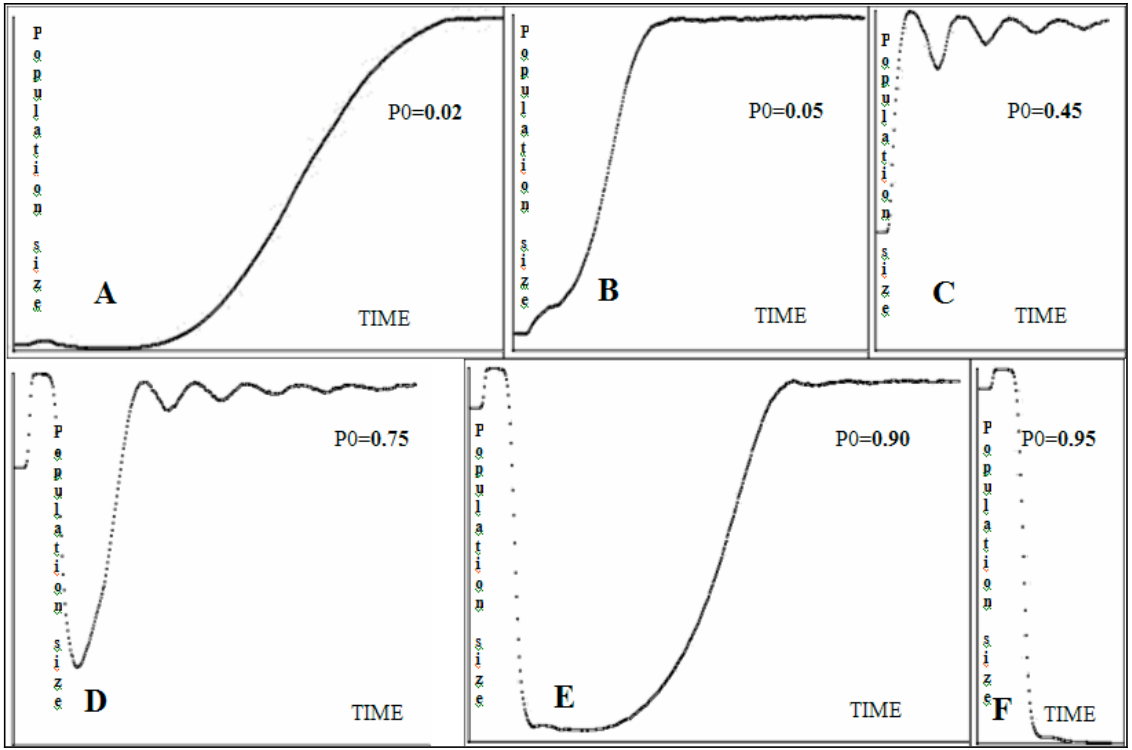
\includegraphics[width=.5\textwidth]{../artigo/imagens/crescimento-populacao-no-tempo}
\caption{Cenários do crescimento populacional no tempo variando P0 (tamanho 
da população inicial). A simulação foi iniciada assumindo que todos os 
indivíduos são "jovens". A rede CA de tamanho 100x100 foi simulado 
\cite{dzwinel:04}.}
\label{fig:crescimento-populacao-no-tempo}
\end{figure}
\end{frame}

\begin{frame}{Proposta}
	\begin{itemize}
		\item Modificação na escolha dos vizinhos.
	\end{itemize}
\begin{figure}[h!]
\centering
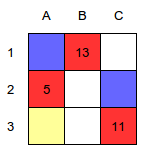
\includegraphics[width=.5\textwidth]{../artigo/imagens/escolha-melhor-vizinho}
\caption{Exemplo de seleção do melhor vizinho.}
\label{fig:busca-tabu}
\end{figure}
\end{frame}

\begin{frame}{Proposta}
	\begin{itemize}
		\item Armazenado na lista Tabu.
	\end{itemize}
\begin{figure}[h!]
\centering
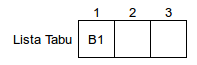
\includegraphics[width=.5\textwidth]{../artigo/imagens/lista-tabu}
\caption{Exemplo da lista Tabu.}
\label{fig:busca-tabu}
\end{figure}
\end{frame}

% ----------------------------------------------------------------------------
% Resultados Alcançados
% ----------------------------------------------------------------------------
\section{Resultados Alcançados}
\begin{frame}{Resultados Alcançados}
%\frametitle{Resultados Alcançados}
	\begin{itemize}
		\item Os parâmetros utilizados neste trabalho foram os mesmos de
		Dzwinel.
	\end{itemize}
\begin{table}[ht]
\centering
\caption{Parametro de uma simulação tipica \cite{dzwinel:04}.}
\label{tab:parametro-simulacao}
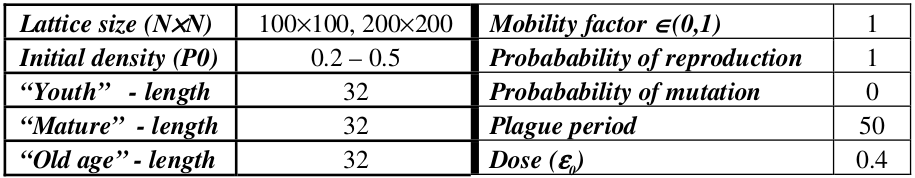
\includegraphics[width=.7\textwidth]{../artigo/imagens/parametro-simulacao}
\end{table}
\end{frame}

\begin{frame}{Resultados Alcançados}
	\begin{itemize}
		\item Os parâmetros utilizados neste trabalho foram os mesmos de
		Dzwinel.
	\end{itemize}
\end{frame}

% ----------------------------------------------------------------------------
% Conclusões
% ----------------------------------------------------------------------------
\section{Conclusões}
\begin{frame}{Conclusões}
%\frametitle
\end{frame}


% ----------------------------------------------------------------------------
% Referências
% ----------------------------------------------------------------------------
\begin{frame}{Referências}
\bibliographystyle{../artigo/sbc}
\bibliography{../artigo/se-alexandre}
\end{frame}

% ----------------------------------------------------------------------------
% Slide de Final
% ----------------------------------------------------------------------------
\begin{frame}
\maketitle
\end{frame}

\end{document}
